\section{Deployment View}
This part of the \emph{Design Document} is devoted to explain at the best the four tiers that compose the \emph{Travlendar+} system.

First of all, the application is created to work either on a web browser or on a mobile phone through an application.
To have a system which is easily maintainable, both the clients will implement the \emph{REST} protocol, with an \emph{HTTPS} communication, in this way the mobile application and the web server can change their internal components, and the only thing to take into account is to implement the correct \emph{RESTful} services.

The clients sends requests to the \emph{Travlendar+} web server, in which there is the \emph{Server Façade}, a component use to receive messages from the Internet and to send them to the \emph{Application Server}.

The \emph{Application Server} is the server that contains all the \emph{Business Logic} components. This layer runs the main functionalities of the \emph{Travlendar+}, and also is used to access to the internal database, to store useful user's data. Notice that the \emph{Application Server} is in a \emph{demilitarized} zone (DMZ), in order to improve security. In this zone is placed also the \emph{Database Server}, in this way the important data are stored in a secure way.

Finally the \emph{Application Server} is also used to communicate with the \emph{External Services}. These services are helpful to the core features of \emph{Travlendar+}. Indeed, the application needs to know the best travel between two tasks, with additional information (such as the estimated travel time and the expected traffic); the travel means, with their time tables, and finally the various tickets' costs.

\subsection{Tier architecture}
As seen before, \emph{Travlendar+} relies on a four tier architecture. This choice surely both increases the overall cost of deployment (in terms of money or time) and the maintenance cost, but is surely useful in terms of the main software attributes as described in the \emph{RASD} Document, which are:
\begin{itemize}
    \item \textbf{Security}: the aim of this architecture is to protect both data and Business Logic from malicious intrusions. The way this requirement is accomplished is by using two "access" servers to the local network which hosts the Application: the \emph{Application Server Façade} and the \emph{External Services Server}. These two machines are protected each one by a firewall who denies access to all connection except the ones coming to the HTTPS port and the ones used by the APIs. In this situation is simpler to imagine these two servers as separate machines, but it is also possible to host the relative software components under a single machine. In both ways, the fact that the local area network is not directly accessible from the world wide web is accomplished.
    
    \item \textbf{Scalability}: using a four tier architecture, we clearly distinguish machines devoted to communication with the web (for example, the web server that communicates with the client), machines devoted to operations and business logic, and machines devoted to data. This means that is fairly simple to expand the network who deals about business logic features without changing the network interfaces to the world wide web: for example, it can be useful to add more services devoted to Business Logic when a certain amount of active users is reached. In this way, there's no need to modify the entire architecture to do it, but only the components who interface themselves to the business logic. 
\end{itemize}
\begin{figure}[H]
    \centering
    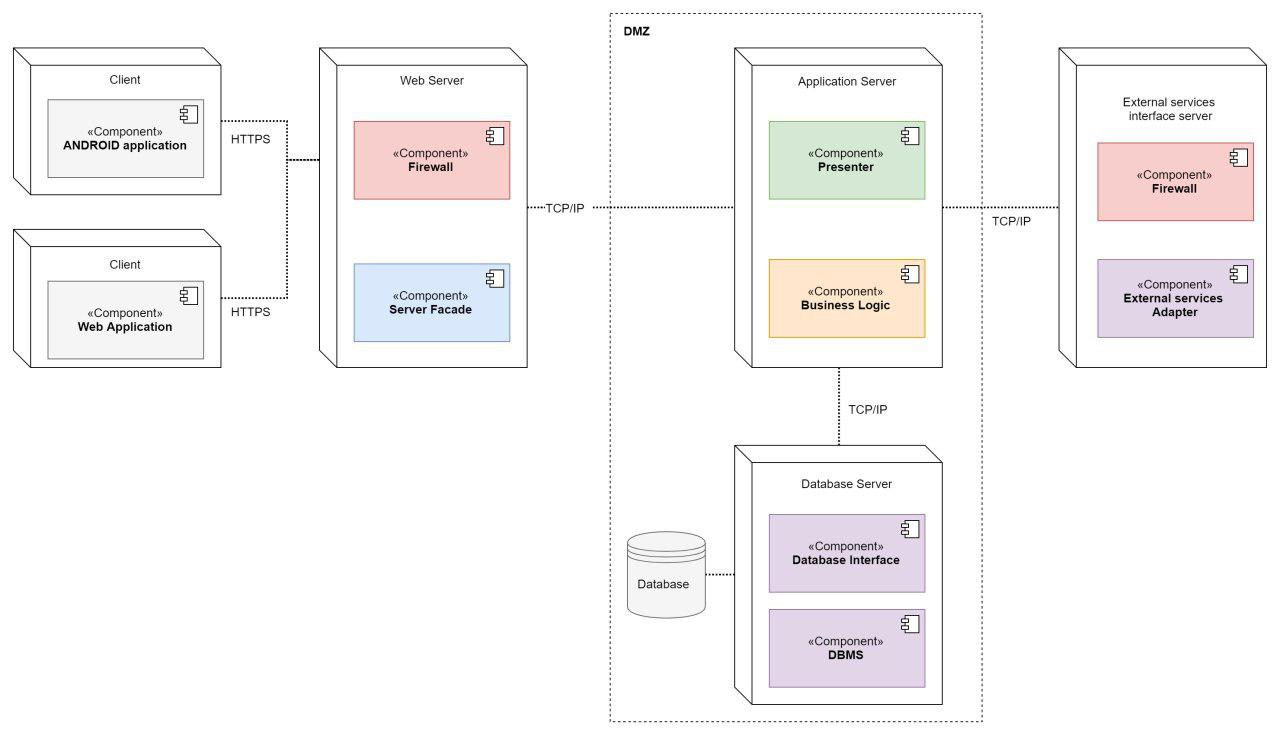
\includegraphics[scale=0.9]{Pictures/DeploymentPictures/deploymentDiagram.jpg}
    \caption{Deployment Diagram for \emph{Travlendar+} System}
\end{figure}
\subsection{Back-end infrastructure}
The back-end infrastructure will be, as described in the \emph{RASD} Document, based on server powered by a UNIX operating system, for example GNU/Linux or Free BSD: these operating systems are well known as great platform when dealing with web and application servers. Moreover, it is important to specify what approach can be used in order to expand the infrastructure when a certain number of active users is reached. A possible way for expanding the platform is to build a server farm containing several clones of the application server; these can work each one on a certain number of requests, so that the whole system is easily upgradable but also fault tolerant. Nonetheless, nowadays several container services are available on the market: these services takes care of the physical structure of the back end infrastructure, leaving to the customer only software maintenance.   
